\documentclass[aspectratio=169]{beamer}

% ── Theme and Colors ──────────────────────────────────────
\usetheme{default}
\usecolortheme{default}
\setbeamertemplate{navigation symbols}{}
\setbeamertemplate{footline}[frame number]

% ── Packages ──────────────────────────────────────────────
\usepackage[T1]{fontenc}
\usepackage{lmodern}
\usepackage{graphicx}
\usepackage{xcolor}
\usepackage{tikz}
\usetikzlibrary{arrows.meta,positioning,shapes.geometric,fit,calc,
                decorations.pathreplacing,backgrounds,patterns,trees}
\usepackage{booktabs}
\usepackage{tabularx}

% ── Brand Colors ──────────────────────────────────────────
\definecolor{garnet}{HTML}{73000A}
\definecolor{rose}{HTML}{CC2E40}
\definecolor{atlantic}{HTML}{466A9F}
\definecolor{congaree}{HTML}{1F414D}
\definecolor{horseshoe}{HTML}{65780B}
\definecolor{grass}{HTML}{CED318}
\definecolor{honeycomb}{HTML}{A49137}
\definecolor{warmgrey}{HTML}{676156}
\definecolor{sandstorm}{HTML}{FFF2E3}
\definecolor{bk90}{HTML}{363636}
\definecolor{bk70}{HTML}{5C5C5C}
\definecolor{bk50}{HTML}{A2A2A2}
\definecolor{bk30}{HTML}{C7C7C7}
\definecolor{bk10}{HTML}{ECECEC}

% ── Beamer Colors ─────────────────────────────────────────
\setbeamercolor{title}{fg=garnet}
\setbeamercolor{frametitle}{fg=garnet}
\setbeamercolor{structure}{fg=garnet}
\setbeamercolor{item}{fg=garnet}
\setbeamercolor{block title}{bg=garnet,fg=white}
\setbeamercolor{block body}{bg=bk10}

% ── TikZ Styles ───────────────────────────────────────────
\tikzset{
  agentbox/.style={
    rectangle, draw=#1, fill=#1!8, thick,
    minimum width=2.2cm, minimum height=0.8cm,
    font=\small\sffamily, align=center,
    inner sep=4pt
  },
  agentbox/.default=garnet,
  workerbox/.style={
    rectangle, draw=atlantic, fill=atlantic!8, thick,
    minimum width=1.8cm, minimum height=0.7cm,
    font=\small\sffamily, align=center,
    inner sep=3pt
  },
  dataarrow/.style={
    -{Stealth[length=5pt]}, thick, color=#1
  },
  dataarrow/.default=bk70,
  sysprompt/.style={rectangle, draw=rose, dashed, fill=rose!5, thick,
    minimum width=2.0cm, minimum height=0.6cm,
    font=\small\sffamily, align=center, inner sep=3pt},
  tooldef/.style={rectangle, draw=atlantic, fill=atlantic!8, thick,
    minimum width=1.8cm, minimum height=0.6cm,
    font=\small\sffamily, align=center, inner sep=3pt},
  wrapperbox/.style={rectangle, draw=garnet, dashed, thick, fill=garnet!3,
    inner sep=8pt},
  pbar/.style={rectangle, draw=#1, fill=#1!30, thick,
    minimum height=0.3cm, font=\scriptsize\sffamily},
  pbar/.default=horseshoe,
  flag/.style={rectangle, draw=rose, fill=rose!15, thick,
    minimum width=0.8cm, minimum height=0.4cm,
    font=\tiny\sffamily\bfseries},
  failbox/.style={rectangle, draw=rose, fill=rose!10, thick,
    font=\small\sffamily, align=center, inner sep=4pt},
  codebox/.style={rectangle, draw=bk70, fill=bk90, text=white,
    font=\ttfamily\small, inner sep=6pt, align=left, text width=#1},
  codebox/.default=6cm,
}

% ══════════════════════════════════════════════════════════
\title{\textcolor{garnet}{\textbf{From LLMs to Multi-Agent Systems}}}
\subtitle{A Progressive Guide to Agent Architectures}
\author{J.C.\ Vaught}
\institute{University of South Carolina}
\date{\today}

\begin{document}

% ── Title ─────────────────────────────────────────────────
\begin{frame}
\titlepage
\end{frame}

% ── Outline ───────────────────────────────────────────────
\begin{frame}{Outline}
\tableofcontents
\end{frame}

% ══════════════════════════════════════════════════════════
\section{Foundation}
% ══════════════════════════════════════════════════════════

\begin{frame}{What Is an LLM?}
\begin{itemize}
    \item Text in, text out --- a prediction engine
    \item No persistent memory between conversations
    \item System prompt shapes behavior (invisible to user)
    \item Size-capability tradeoff: small/fast vs.\ large/capable
\end{itemize}
\end{frame}

\begin{frame}{LLM: Basic Interface}
\centering
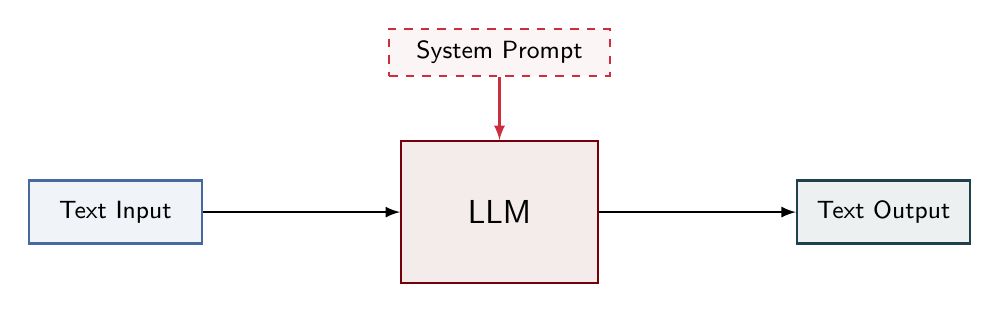
\begin{tikzpicture}[node distance=1.5cm and 2.5cm]
    \node[agentbox=atlantic] (textin1) {Text Input};
    \node[agentbox, right=of textin1, minimum width=2.5cm, minimum height=1.8cm] (llm1) {\large LLM};
    \node[agentbox=congaree, right=of llm1] (textout1) {Text Output};
    \node[sysprompt, above=0.8cm of llm1, minimum width=2.8cm] (sysprompt1) {System Prompt};
    \draw[-latex, rose, thick] (sysprompt1) -- (llm1);
    \draw[-latex, thick] (textin1) -- (llm1);
    \draw[-latex, thick] (llm1) -- (textout1);
\end{tikzpicture}
\end{frame}

\begin{frame}{Multimodal LLM}
\centering
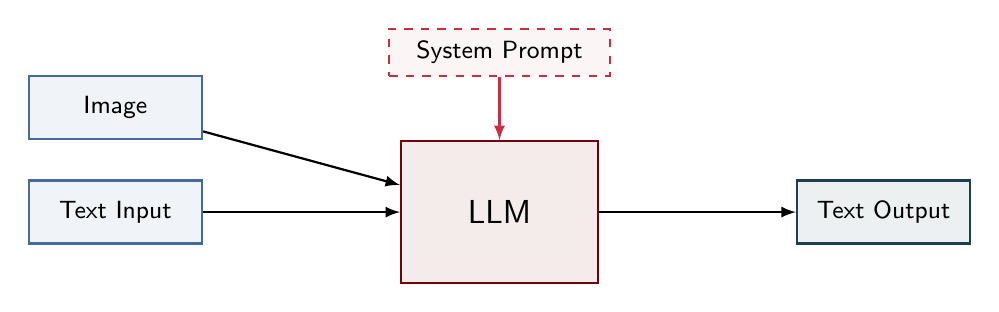
\begin{tikzpicture}[node distance=1.5cm and 2.5cm]
    \node[agentbox=atlantic] (image2) {Image};
    \node[agentbox=atlantic, below=0.5cm of image2] (textin2) {Text Input};
    \node[agentbox, right=of textin2, minimum width=2.5cm, minimum height=1.8cm] (llm2) {\large LLM};
    \node[agentbox=congaree, right=of llm2] (textout2) {Text Output};
    \node[sysprompt, above=0.8cm of llm2, minimum width=2.8cm] (sysprompt2) {System Prompt};
    \draw[-latex, rose, thick] (sysprompt2) -- (llm2);
    \draw[-latex, thick] (image2) -- (llm2);
    \draw[-latex, thick] (textin2) -- (llm2);
    \draw[-latex, thick] (llm2) -- (textout2);
\end{tikzpicture}

\vspace{0.5cm}
\small Can see images, but output is still text only
\end{frame}

\begin{frame}{AI-Assisted Coding (Autocomplete)}
\begin{itemize}
    \item LLM predicts code continuation
    \item No access to other files, tools, or execution
    \item User accepts or ignores suggestions
\end{itemize}

\vspace{0.5cm}
\centering
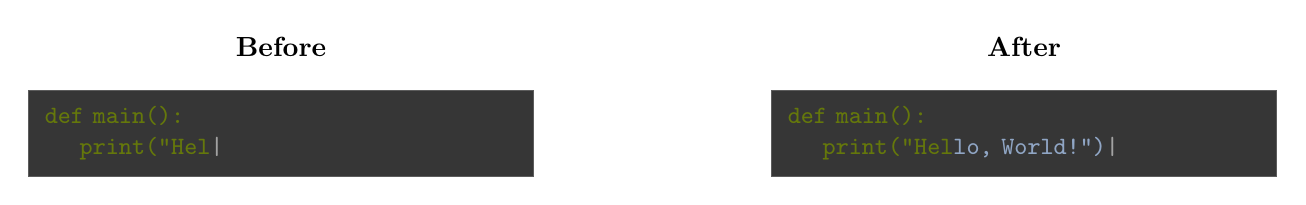
\begin{tikzpicture}[node distance=1.2cm]
    \node[codebox] (before) {%
        \textcolor{horseshoe}{\texttt{def main():}}\\
        \textcolor{horseshoe}{\texttt{~~~~print("Hel}}\textcolor{bk50}{|}%
    };
    \node[above=0.3cm of before, font=\bfseries] {Before};
    \node[codebox, right=3cm of before] (after) {%
        \textcolor{horseshoe}{\texttt{def main():}}\\
        \textcolor{horseshoe}{\texttt{~~~~print("Hel}}\textcolor{atlantic!60!white}{\texttt{lo, World!")}}\textcolor{bk50}{|}%
    };
    \node[above=0.3cm of after, font=\bfseries] {After};
\end{tikzpicture}
\end{frame}

\begin{frame}{What Is an AI Coding Agent?}
\begin{itemize}
    \item LLM + wrapper program = agent
    \item Wrapper provides: tool definitions + execution environment
    \item LLM outputs tool calls $\to$ wrapper executes $\to$ results fed back
    \item Creates an action loop until task complete
\end{itemize}
\end{frame}

\begin{frame}{Agent Architecture}
\centering
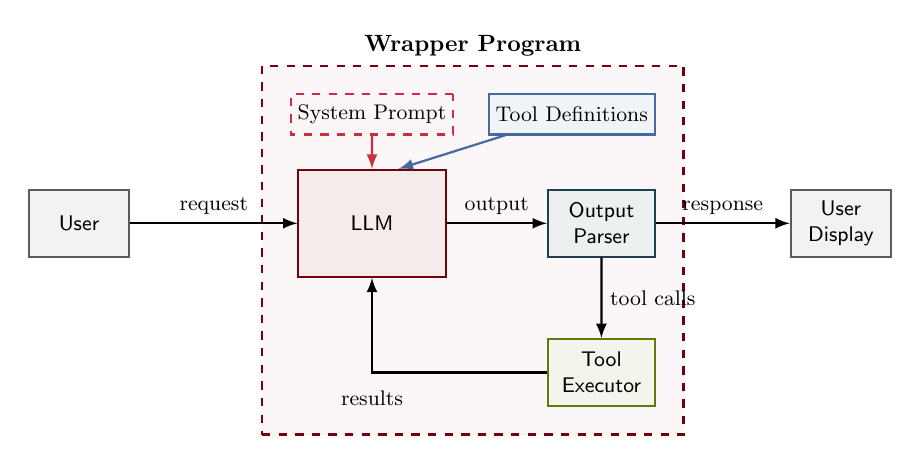
\begin{tikzpicture}[node distance=1.0cm and 1.5cm, >={Latex[length=2mm]}, scale=0.85, transform shape]
    \node[agentbox=bk70, minimum width=1.5cm, minimum height=1cm] (user) {User};
    \node[agentbox, right=2.5cm of user, minimum width=2.2cm, minimum height=1.6cm] (llm) {LLM};
    \node[sysprompt, above=0.5cm of llm, minimum width=2.2cm, font=\small] (sysprompt) {System Prompt};
    \node[tooldef, right=0.5cm of sysprompt, minimum width=2cm, font=\small] (tooldef) {Tool Definitions};
    \draw[-latex, rose, thick] (sysprompt) -- (llm);
    \draw[-latex, atlantic, thick] (tooldef) -- ([xshift=0.4cm]llm.north);
    \node[agentbox=congaree, right=of llm, minimum width=1.6cm, minimum height=1cm] (parser) {Output\\Parser};
    \node[agentbox=horseshoe, below=1.2cm of parser, minimum width=1.6cm, minimum height=1cm] (executor) {Tool\\Executor};
    \node[agentbox=bk70, right=2cm of parser, minimum width=1.5cm, minimum height=1cm] (display) {User\\Display};
    \begin{scope}[on background layer]
      \node[wrapperbox, fit=(sysprompt)(tooldef)(llm)(parser)(executor), inner sep=10pt] (wrapper) {};
    \end{scope}
    \node[above=0cm of wrapper.north, font=\bfseries] {Wrapper Program};
    \draw[-latex, thick] (user) -- (llm) node[midway, above, font=\small] {request};
    \draw[-latex, thick] (llm) -- (parser) node[midway, above, font=\small] {output};
    \draw[-latex, thick] (parser) -- (executor) node[midway, right, font=\small] {tool calls};
    \draw[-latex, thick] (parser) -- (display) node[midway, above, font=\small] {response};
    \draw[-latex, thick] (executor.west) -- (executor.west -| llm.south) -- (llm.south) node[pos=-0.1, below, font=\small] {results};
\end{tikzpicture}
\end{frame}

% ══════════════════════════════════════════════════════════
\section{Agent Workflows}
% ══════════════════════════════════════════════════════════

\begin{frame}{Three Execution Models}
\begin{itemize}
    \item \textbf{Streaming:} Execute tools as soon as detected mid-generation
    \item \textbf{Batch:} Generate full response, then execute all tools
    \item \textbf{Parallel:} Some tools run concurrently, others block
\end{itemize}
\end{frame}

\begin{frame}{Streaming Execution}
\centering
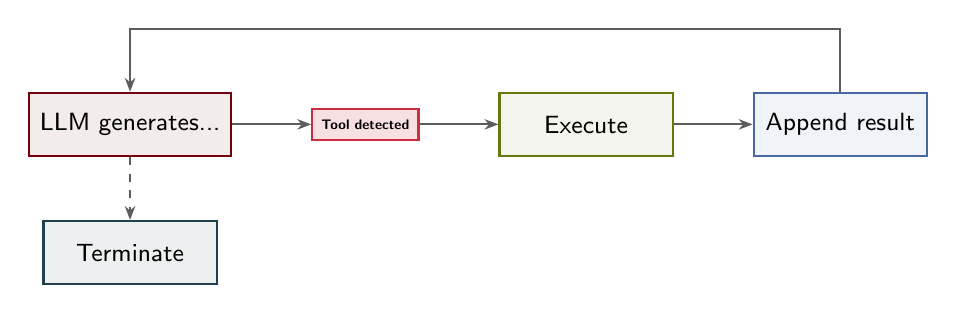
\begin{tikzpicture}[node distance=1.2cm and 1.0cm]
\node[agentbox] (llm1) {LLM generates...};
\node[flag, right=of llm1] (detect) {Tool detected};
\node[agentbox=horseshoe, right=of detect] (exec) {Execute};
\node[agentbox=atlantic, right=of exec] (append) {Append result};
\node[agentbox=congaree, below=0.8cm of llm1] (term1) {Terminate};
\draw[dataarrow] (llm1) -- (detect);
\draw[dataarrow] (detect) -- (exec);
\draw[dataarrow] (exec) -- (append);
\draw[dataarrow] (append.north) -- ++(0,0.8) -| (llm1.north);
\draw[dataarrow, dashed] (llm1) -- (term1);
\end{tikzpicture}

\vspace{0.3cm}
\small Real-time, responsive --- tools fire immediately
\end{frame}

\begin{frame}{Batch Execution}
\centering
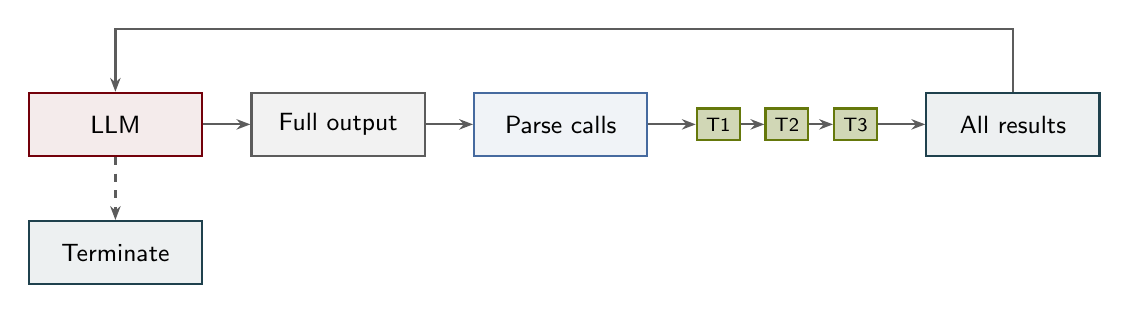
\begin{tikzpicture}[node distance=0.6cm and 0.6cm]
\node[agentbox] (llm2) {LLM};
\node[agentbox=bk70, right=of llm2] (output) {Full output};
\node[agentbox=atlantic, right=of output] (parse) {Parse calls};
\node[pbar, right=of parse] (t1) {T1};
\node[pbar, right=0.3cm of t1] (t2) {T2};
\node[pbar, right=0.3cm of t2] (t3) {T3};
\node[agentbox=congaree, right=of t3] (allres) {All results};
\node[agentbox=congaree, below=0.8cm of llm2] (term2) {Terminate};
\draw[dataarrow, dashed] (llm2) -- (term2);
\draw[dataarrow] (llm2) -- (output);
\draw[dataarrow] (output) -- (parse);
\draw[dataarrow] (parse) -- (t1);
\draw[dataarrow] (t1) -- (t2);
\draw[dataarrow] (t2) -- (t3);
\draw[dataarrow] (t3) -- (allres);
\draw[dataarrow] (allres.north) -- ++(0,0.8) -| (llm2.north);
\end{tikzpicture}

\vspace{0.3cm}
\small Simpler to implement --- classic chatbot model
\end{frame}

\begin{frame}{Parallel Execution}
\centering
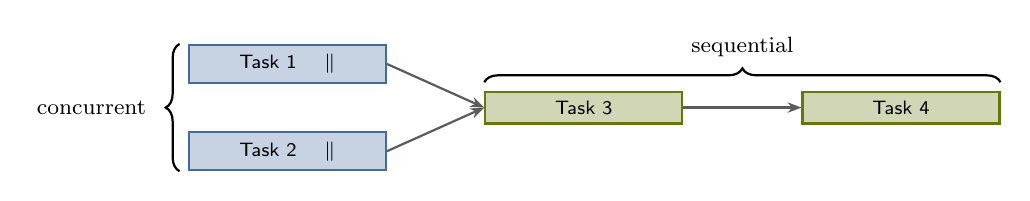
\begin{tikzpicture}[node distance=1.0cm and 1.5cm]
\node[pbar=atlantic, minimum width=2.5cm] (t1) {Task 1 \quad $\parallel$};
\node[pbar=atlantic, minimum width=2.5cm, below=0.6cm of t1] (t2) {Task 2 \quad $\parallel$};
\node[pbar=horseshoe, minimum width=2.5cm, right=2.5cm of $(t1)!0.5!(t2)$] (t3) {Task 3};
\node[pbar=horseshoe, minimum width=2.5cm, right=1.5cm of t3] (t4) {Task 4};
\draw[dataarrow] (t1.east) -- (t3.west);
\draw[dataarrow] (t2.east) -- (t3.west);
\draw[dataarrow] (t3) -- (t4);
\draw[thick, decorate, decoration={brace, amplitude=5pt, mirror, raise=3pt}]
  (t1.north west) -- (t2.south west)
  node[midway, left=0.4cm, font=\footnotesize, align=center] {concurrent};
\draw[thick, decorate, decoration={brace, amplitude=5pt, raise=3pt}]
  (t3.north west) -- (t4.north east)
  node[midway, above=0.3cm, font=\footnotesize, align=center] {sequential};
\end{tikzpicture}

\vspace{0.3cm}
\small Independent tasks overlap; blocking tasks wait
\end{frame}

% ══════════════════════════════════════════════════════════
\section{Slaves and Masters}
% ══════════════════════════════════════════════════════════

\begin{frame}{What Is a Slave?}
\begin{itemize}
    \item Same architecture as an agent
    \item Called by another agent (master), not by a human
    \item Often uses smaller/specialized model
    \item Scoped tools and specialized system prompt
\end{itemize}
\end{frame}

\begin{frame}{Master vs.\ Slave}
\centering
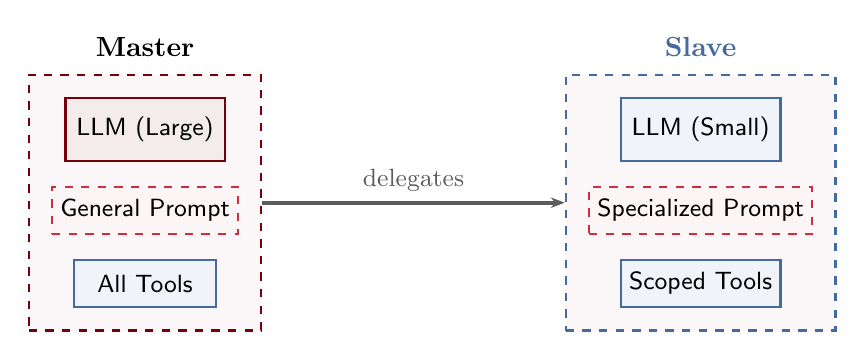
\begin{tikzpicture}[node distance=0.3cm and 1.5cm]
\node[agentbox, minimum width=2cm] (parent-llm) {LLM (Large)};
\node[sysprompt, below=of parent-llm] (parent-prompt) {General Prompt};
\node[tooldef, below=of parent-prompt] (parent-tools) {All Tools};
\node[agentbox=atlantic, minimum width=2cm, right=5cm of parent-llm] (child-llm) {LLM (Small)};
\node[sysprompt, below=of child-llm] (child-prompt) {Specialized Prompt};
\node[tooldef, below=of child-prompt] (child-tools) {Scoped Tools};
\begin{scope}[on background layer]
  \node[wrapperbox, draw=garnet, dashed, fit=(parent-llm)(parent-prompt)(parent-tools), inner sep=8pt] (parent-wrapper) {};
  \node[wrapperbox, draw=atlantic, dashed, fit=(child-llm)(child-prompt)(child-tools), inner sep=8pt] (child-wrapper) {};
\end{scope}
\node[above=0.1cm of parent-wrapper.north, font=\bfseries] {Master};
\node[above=0.1cm of child-wrapper.north, font=\bfseries, text=atlantic] {Slave};
\draw[dataarrow, line width=1.5pt] (parent-wrapper.east) -- (child-wrapper.west)
  node[midway, above, font=\small] {delegates};
\end{tikzpicture}
\end{frame}

\begin{frame}{Slave Lifecycle}
\centering
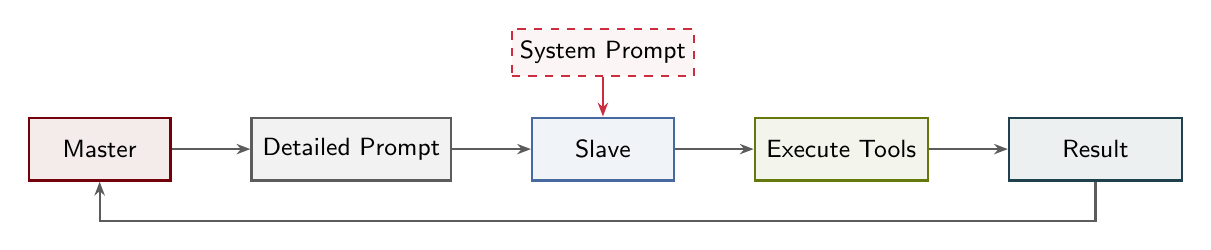
\begin{tikzpicture}[node distance=0.7cm and 1.0cm]
\node[agentbox, minimum width=1.8cm] (parent) {Master};
\node[agentbox=bk70, right=of parent] (prompt) {Detailed Prompt};
\node[agentbox=atlantic, right=of prompt, minimum width=1.8cm] (subllm) {Slave};
\node[agentbox=horseshoe, right=of subllm] (exec) {Execute Tools};
\node[agentbox=congaree, right=of exec] (result) {Result};
\node[sysprompt, above=0.5cm of subllm] (sysp) {System Prompt};
\draw[dataarrow=rose] (sysp) -- (subllm);
\draw[dataarrow] (parent) -- (prompt);
\draw[dataarrow] (prompt) -- (subllm);
\draw[dataarrow] (subllm) -- (exec);
\draw[dataarrow] (exec) -- (result);
\draw[dataarrow] (result.south) -- ++(0,-0.5) -| (parent.south);
\end{tikzpicture}
\end{frame}

\begin{frame}{Master-Slave Pattern}
\centering
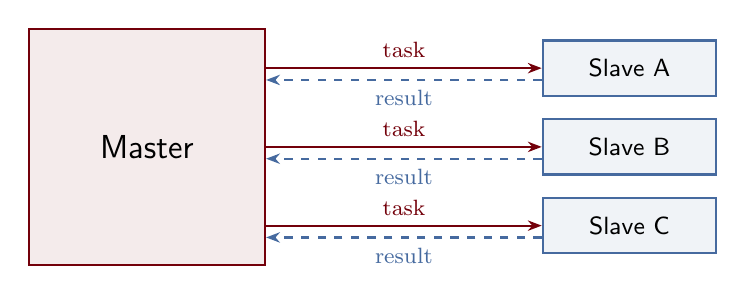
\begin{tikzpicture}[node distance=0.6cm]
\node[agentbox=garnet, minimum width=3cm, minimum height=3cm] (master) {\large Master};
\node[workerbox, right=3.5cm of master, yshift=1cm, minimum width=2.2cm] (w1) {Slave A};
\node[workerbox, right=3.5cm of master, yshift=0.0cm, minimum width=2.2cm] (w2) {Slave B};
\node[workerbox, right=3.5cm of master, yshift=-1cm, minimum width=2.2cm] (w3) {Slave C};
\draw[dataarrow=garnet] (master.east |- w1) -- (w1.west) node[midway, above, font=\footnotesize] {task};
\draw[dataarrow=garnet] (master.east |- w2) -- (w2.west) node[midway, above, font=\footnotesize] {task};
\draw[dataarrow=garnet] (master.east |- w3) -- (w3.west) node[midway, above, font=\footnotesize] {task};
\draw[dataarrow=atlantic, dashed] ([yshift=-0.15cm]w1.west) -- ([yshift=-0.15cm]master.east |- w1) node[midway, below, font=\footnotesize] {result};
\draw[dataarrow=atlantic, dashed] ([yshift=-0.15cm]w2.west) -- ([yshift=-0.15cm]master.east |- w2) node[midway, below, font=\footnotesize] {result};
\draw[dataarrow=atlantic, dashed] ([yshift=-0.15cm]w3.west) -- ([yshift=-0.15cm]master.east |- w3) node[midway, below, font=\footnotesize] {result};
\end{tikzpicture}
\end{frame}

% ══════════════════════════════════════════════════════════
\section{Communication Patterns}
% ══════════════════════════════════════════════════════════

\begin{frame}{Communication: Direct Return}
\centering
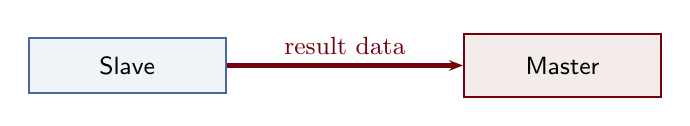
\begin{tikzpicture}[node distance=1.2cm and 2.5cm]
\node[workerbox, minimum width=2.5cm] (w1) {Slave};
\node[agentbox, right=3cm of w1, minimum width=2.5cm] (m1) {Master};
\draw[dataarrow=garnet, line width=1.5pt] (w1) -- (m1) node[midway, above, font=\small] {result data};
\end{tikzpicture}

\vspace{0.5cm}
\small Result embedded in completion message\\
Best for small results (pass/fail, status codes)
\end{frame}

\begin{frame}{Communication: File-Mediated}
\centering
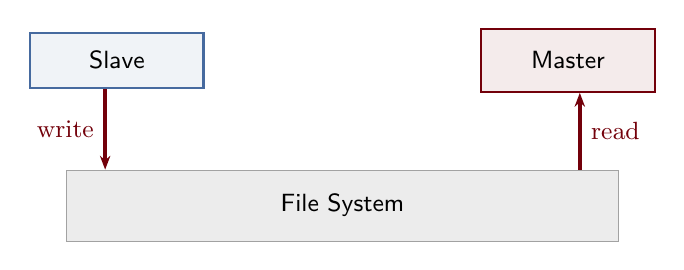
\begin{tikzpicture}[node distance=1.0cm and 1.5cm]
\node[workerbox, minimum width=2.2cm] (w2) {Slave};
\node[agentbox, right=3.5cm of w2, minimum width=2.2cm] (m2) {Master};
\node[rectangle, draw=bk50, fill=bk10, minimum width=7cm, minimum height=0.9cm,
  below=1cm of $(w2.south)!0.5!(m2.south)$, font=\small\sffamily] (file) {File System};
\draw[dataarrow=garnet, line width=1.5pt] ([xshift=-0.15cm]w2.south) -- ([xshift=-0.15cm]w2.south |- file.north) node[midway, left, font=\small] {write};
\draw[dataarrow=garnet, line width=1.5pt] ([xshift=0.15cm]m2.south |- file.north) -- ([xshift=0.15cm]m2.south) node[midway, right, font=\small] {read};
\end{tikzpicture}

\vspace{0.3cm}
\small Best for large artifacts, binaries, generated files
\end{frame}

\begin{frame}{Communication: Hybrid (Most Common)}
\centering
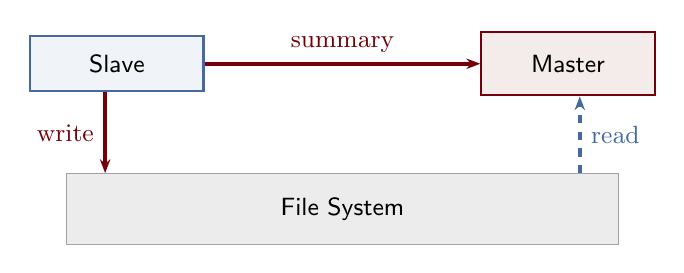
\begin{tikzpicture}[node distance=1.0cm and 1.5cm]
\node[workerbox, minimum width=2.2cm] (w3) {Slave};
\node[agentbox, right=3.5cm of w3, minimum width=2.2cm] (m3) {Master};
\node[rectangle, draw=bk50, fill=bk10, minimum width=7cm, minimum height=0.9cm,
  below=1cm of $(w3.south)!0.5!(m3.south)$, font=\small\sffamily] (file3) {File System};
\draw[dataarrow=garnet, line width=1.5pt] ([xshift=-0.15cm]w3.south) -- ([xshift=-0.15cm]w3.south |- file3.north) node[midway, left, font=\small] {write};
\draw[dataarrow=atlantic, dashed, line width=1.5pt] ([xshift=0.15cm]m3.south |- file3.north) -- ([xshift=0.15cm]m3.south) node[midway, right, font=\small] {read};
\draw[dataarrow=garnet, line width=1.5pt] (w3) -- (m3) node[midway, above, font=\small] {summary};
\end{tikzpicture}

\vspace{0.3cm}
\small Detailed artifacts to disk + summary to master\\
Example: ``14 passed, 2 failed'' + full logs on disk
\end{frame}

% ══════════════════════════════════════════════════════════
\section{Control Models}
% ══════════════════════════════════════════════════════════

\begin{frame}{Imperative vs.\ Declarative Control}
\centering
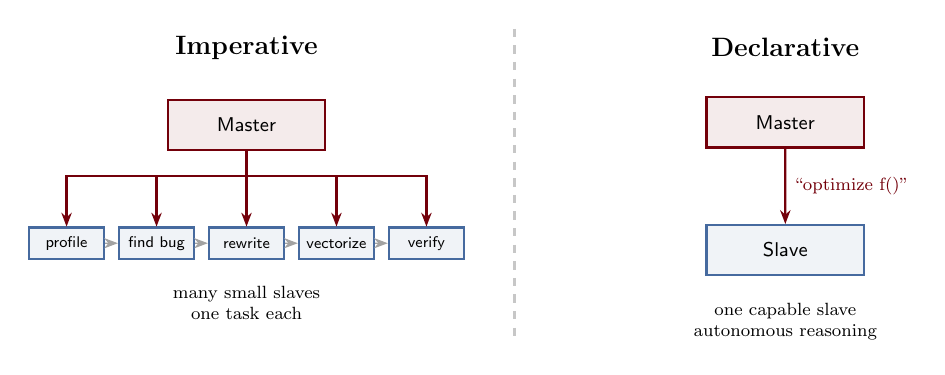
\begin{tikzpicture}[node distance=0.4cm and 0.6cm, scale=0.8, transform shape]
% Imperative
\node[font=\large\bfseries] (imp-title) {Imperative};
\node[agentbox=garnet, below=0.5cm of imp-title, minimum width=2.5cm] (imp-orch) {Master};
\node[workerbox, below=1.2cm of imp-orch, minimum width=1.2cm, minimum height=0.5cm, font=\scriptsize\sffamily] (iw3) {rewrite};
\node[workerbox, left=0.2cm of iw3, minimum width=1.2cm, minimum height=0.5cm, font=\scriptsize\sffamily] (iw2) {find bug};
\node[workerbox, left=0.2cm of iw2, minimum width=1.2cm, minimum height=0.5cm, font=\scriptsize\sffamily] (iw1) {profile};
\node[workerbox, right=0.2cm of iw3, minimum width=1.2cm, minimum height=0.5cm, font=\scriptsize\sffamily] (iw4) {vectorize};
\node[workerbox, right=0.2cm of iw4, minimum width=1.2cm, minimum height=0.5cm, font=\scriptsize\sffamily] (iw5) {verify};
\draw[dataarrow=garnet] (imp-orch.south) -- ++(0,-0.4) -| (iw1.north);
\draw[dataarrow=garnet] (imp-orch.south) -- ++(0,-0.4) -| (iw2.north);
\draw[dataarrow=garnet] (imp-orch.south) -- ++(0,-0.4) -| (iw3.north);
\draw[dataarrow=garnet] (imp-orch.south) -- ++(0,-0.4) -| (iw4.north);
\draw[dataarrow=garnet] (imp-orch.south) -- ++(0,-0.4) -| (iw5.north);
\draw[dataarrow=bk50, thin] (iw1.east) -- (iw2.west);
\draw[dataarrow=bk50, thin] (iw2.east) -- (iw3.west);
\draw[dataarrow=bk50, thin] (iw3.east) -- (iw4.west);
\draw[dataarrow=bk50, thin] (iw4.east) -- (iw5.west);
\node[font=\footnotesize, below=0.3cm of iw3, align=center] {many small slaves\\one task each};

% Declarative
\node[font=\large\bfseries, right=6cm of imp-title] (dec-title) {Declarative};
\node[agentbox=garnet, below=0.5cm of dec-title, minimum width=2.5cm] (dec-orch) {Master};
\node[agentbox=atlantic, below=1.2cm of dec-orch, minimum width=2.5cm] (dw1) {Slave};
\draw[dataarrow=garnet] (dec-orch) -- (dw1) node[midway, right, font=\footnotesize] {``optimize f()''};
\node[font=\footnotesize, below=0.3cm of dw1, align=center] {one capable slave\\autonomous reasoning};

% Separator
\draw[dashed, bk30, thick] ($(imp-title.east)!0.5!(dec-title.west)$) ++(0,0.3) -- ++(0,-5);
\end{tikzpicture}
\end{frame}

\begin{frame}{Control Model Comparison}
\centering
\small
\begin{tabular}{lccc}
\toprule
\textbf{Property} & \textbf{Imperative} & \textbf{Declarative} & \textbf{Hybrid} \\
\midrule
Intelligence location & Master & Slave & Shared \\
Slave autonomy & Low & High & Medium \\
Predictability & High & Low & Medium \\
Flexibility & Low & High & Medium \\
\bottomrule
\end{tabular}
\end{frame}

% ══════════════════════════════════════════════════════════
\section{Orchestration Cycles}
% ══════════════════════════════════════════════════════════

\begin{frame}{The Master Cycle}
\begin{itemize}
    \item Five-step loop: \textbf{Plan} $\to$ \textbf{Delegate} $\to$ \textbf{Wait} $\to$ \textbf{Collect} $\to$ \textbf{Decide}
    \item Differences lie in how each step executes
    \item May traverse once (single-pass) or repeat (iterative)
\end{itemize}
\end{frame}

\begin{frame}{Single-Pass Orchestration}
\centering
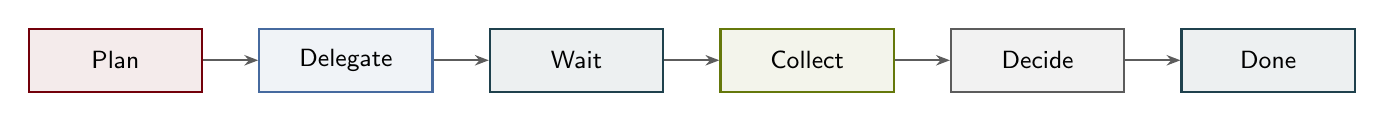
\begin{tikzpicture}[node distance=0.7cm and 0.7cm]
  \node[agentbox] (p1) {Plan};
  \node[agentbox=atlantic, right=of p1] (d1) {Delegate};
  \node[agentbox=congaree, right=of d1] (w1) {Wait};
  \node[agentbox=horseshoe, right=of w1] (c1) {Collect};
  \node[agentbox=bk70, right=of c1] (de1) {Decide};
  \node[agentbox=congaree, right=of de1] (done1) {Done};
  \draw[dataarrow] (p1) -- (d1);
  \draw[dataarrow] (d1) -- (w1);
  \draw[dataarrow] (w1) -- (c1);
  \draw[dataarrow] (c1) -- (de1);
  \draw[dataarrow] (de1) -- (done1);
\end{tikzpicture}

\vspace{0.5cm}
\small One traversal, no recovery, no refinement\\
If initial plan is wrong, no recourse
\end{frame}

\begin{frame}{Iterative Orchestration}
\centering
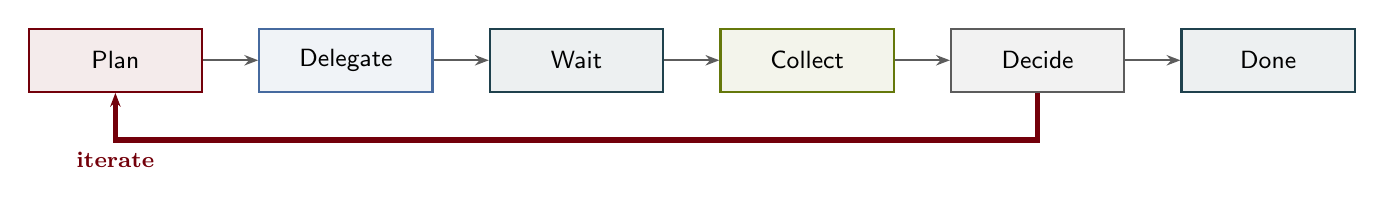
\begin{tikzpicture}[node distance=0.7cm and 0.7cm]
  \node[agentbox] (p2) {Plan};
  \node[agentbox=atlantic, right=of p2] (d2) {Delegate};
  \node[agentbox=congaree, right=of d2] (w2) {Wait};
  \node[agentbox=horseshoe, right=of w2] (c2) {Collect};
  \node[agentbox=bk70, right=of c2] (de2) {Decide};
  \node[agentbox=congaree, right=of de2] (done2) {Done};
  \draw[dataarrow] (p2) -- (d2);
  \draw[dataarrow] (d2) -- (w2);
  \draw[dataarrow] (w2) -- (c2);
  \draw[dataarrow] (c2) -- (de2);
  \draw[dataarrow] (de2) -- (done2);
  \draw[dataarrow, garnet, line width=2pt]
    (de2.south) -- ++(0,-0.6) -| (p2.south)
    node[pos=0.5, below, font=\footnotesize\bfseries] {iterate};
\end{tikzpicture}

\vspace{0.5cm}
\small Feedback loop enables error recovery and refinement\\
Terminates on: quality threshold, max iterations, or no new tasks
\end{frame}

\begin{frame}{Reactive Orchestration}
\centering
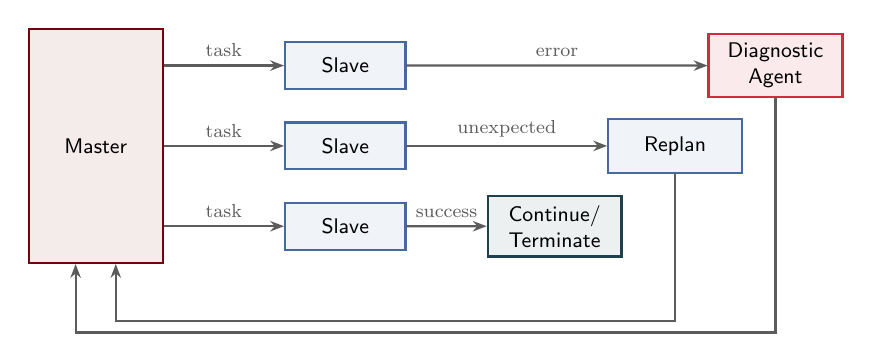
\begin{tikzpicture}[node distance=0.6cm and 0.8cm, scale=0.85, transform shape]
  \node[agentbox, minimum height=3.5cm, minimum width=2cm] (orch) {Master};
  % Error row
  \node[workerbox, right=1.8cm of orch, yshift=1.2cm] (w2) {Slave};
  \node[failbox, right=4.5cm of w2, minimum width=2cm] (diag) {Diagnostic\\Agent};
  \draw[dataarrow] (orch.east |- w2) -- node[above,font=\footnotesize] {task} (w2);
  \draw[dataarrow] (w2) -- node[above,font=\footnotesize] {error} (diag);
  \draw[dataarrow] (diag.south) -- ++(0,-3.5) -| ([xshift=-0.3cm]orch.south);
  % Unexpected row
  \node[workerbox, right=1.8cm of orch] (w3) {Slave};
  \node[agentbox=atlantic, right=3cm of w3, minimum width=2cm] (replan) {Replan};
  \draw[dataarrow] (orch.east |- w3) -- node[above,font=\footnotesize] {task} (w3);
  \draw[dataarrow] (w3) -- node[above,font=\footnotesize] {unexpected} (replan);
  \draw[dataarrow] (replan.south) -- ++(0,-2.2) -| ([xshift=0.3cm]orch.south);
  % Success row
  \node[workerbox, right=1.8cm of orch, yshift=-1.2cm] (w1) {Slave};
  \node[agentbox=congaree, right=1.2cm of w1, minimum width=2cm] (cont) {Continue/\\Terminate};
  \draw[dataarrow] (orch.east |- w1) -- node[above,font=\footnotesize] {task} (w1);
  \draw[dataarrow] (w1) -- node[above,font=\footnotesize] {success} (cont);
\end{tikzpicture}

\vspace{0.2cm}
\small Event-driven: react to success, error, or unexpected discoveries
\end{frame}

% ══════════════════════════════════════════════════════════
\section{Topologies}
% ══════════════════════════════════════════════════════════

\begin{frame}{Parallel Agent Execution: Full Barrier}
\centering
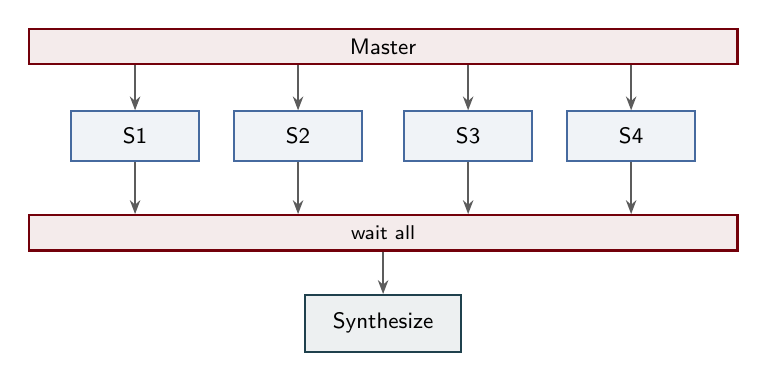
\begin{tikzpicture}[node distance=0.7cm and 0.7cm, scale=0.9, transform shape]
  \node[agentbox=garnet, minimum width=10cm, minimum height=0.5cm] (orch1) {Master};
  \node[workerbox] at ([yshift=-1cm, xshift=-3.5cm]orch1.south) (w11) {S1};
  \node[workerbox] at ([yshift=-1cm, xshift=-1.2cm]orch1.south) (w12) {S2};
  \node[workerbox] at ([yshift=-1cm, xshift=1.2cm]orch1.south)  (w13) {S3};
  \node[workerbox] at ([yshift=-1cm, xshift=3.5cm]orch1.south)  (w14) {S4};
  \foreach \w in {w11,w12,w13,w14} { \draw[dataarrow] (orch1.south -| \w) -- (\w); }
  \node[agentbox=garnet, minimum width=10cm, minimum height=0.5cm] at ([yshift=-1cm]$(w12.south)!0.5!(w13.south)$) (barrier1) {\footnotesize wait all};
  \foreach \w in {w11,w12,w13,w14} { \draw[dataarrow] (\w) -- (barrier1.north -| \w); }
  \node[agentbox=congaree, below=0.6cm of barrier1] (syn1) {Synthesize};
  \draw[dataarrow] (barrier1) -- (syn1);
\end{tikzpicture}

\vspace{0.3cm}
\small Slowest slave determines total time
\end{frame}

\begin{frame}{Parallel Agent Execution: Partial Barrier (k-of-n)}
\centering
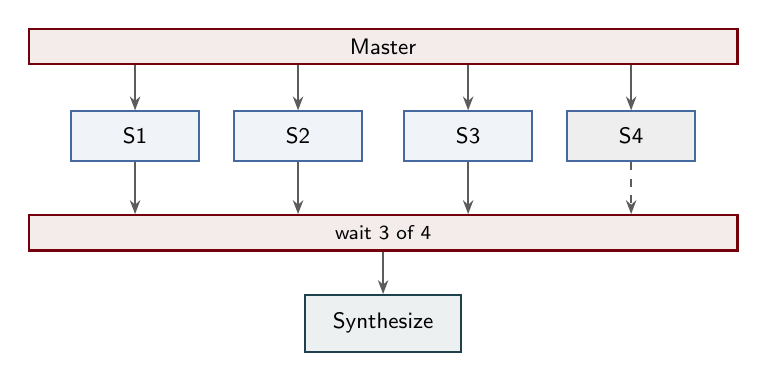
\begin{tikzpicture}[node distance=0.7cm and 0.7cm, scale=0.9, transform shape]
  \node[agentbox=garnet, minimum width=10cm, minimum height=0.5cm] (orch2) {Master};
  \node[workerbox] at ([yshift=-1cm, xshift=-3.5cm]orch2.south) (w21) {S1};
  \node[workerbox] at ([yshift=-1cm, xshift=-1.2cm]orch2.south) (w22) {S2};
  \node[workerbox] at ([yshift=-1cm, xshift=1.2cm]orch2.south)  (w23) {S3};
  \node[workerbox, fill=bk30!30] at ([yshift=-1cm, xshift=3.5cm]orch2.south)  (w24) {S4};
  \foreach \w in {w21,w22,w23,w24} { \draw[dataarrow] (orch2.south -| \w) -- (\w); }
  \node[agentbox=garnet, minimum width=10cm, minimum height=0.5cm] at ([yshift=-1cm]$(w22.south)!0.5!(w23.south)$) (barrier2) {\footnotesize wait 3 of 4};
  \draw[dataarrow] (w21) -- (barrier2.north -| w21);
  \draw[dataarrow] (w22) -- (barrier2.north -| w22);
  \draw[dataarrow] (w23) -- (barrier2.north -| w23);
  \draw[dataarrow, dashed] (w24) -- (barrier2.north -| w24);
  \node[agentbox=congaree, below=0.6cm of barrier2] (syn2) {Synthesize};
  \draw[dataarrow] (barrier2) -- (syn2);
\end{tikzpicture}

\vspace{0.3cm}
\small Proceed when k slaves finish; grayed slave not required
\end{frame}

\begin{frame}{Parallel Agent Execution: Timeout Barrier}
\centering
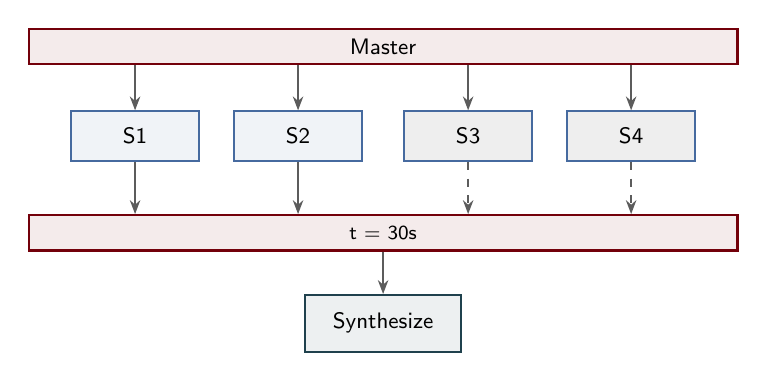
\begin{tikzpicture}[node distance=0.7cm and 0.7cm, scale=0.9, transform shape]
  \node[agentbox=garnet, minimum width=10cm, minimum height=0.5cm] (orch3) {Master};
  \node[workerbox] at ([yshift=-1cm, xshift=-3.5cm]orch3.south) (w31) {S1};
  \node[workerbox] at ([yshift=-1cm, xshift=-1.2cm]orch3.south) (w32) {S2};
  \node[workerbox, fill=bk30!30] at ([yshift=-1cm, xshift=1.2cm]orch3.south)  (w33) {S3};
  \node[workerbox, fill=bk30!30] at ([yshift=-1cm, xshift=3.5cm]orch3.south)  (w34) {S4};
  \foreach \w in {w31,w32,w33,w34} { \draw[dataarrow] (orch3.south -| \w) -- (\w); }
  \node[agentbox=garnet, minimum width=10cm, minimum height=0.5cm] at ([yshift=-1cm]$(w32.south)!0.5!(w33.south)$) (barrier3) {\footnotesize t = 30s};
  \draw[dataarrow] (w31) -- (barrier3.north -| w31);
  \draw[dataarrow] (w32) -- (barrier3.north -| w32);
  \draw[dataarrow, dashed] (w33) -- (barrier3.north -| w33);
  \draw[dataarrow, dashed] (w34) -- (barrier3.north -| w34);
  \node[agentbox=congaree, below=0.6cm of barrier3] (syn3) {Synthesize};
  \draw[dataarrow] (barrier3) -- (syn3);
\end{tikzpicture}

\vspace{0.3cm}
\small Prioritizes responsiveness over completeness
\end{frame}

\begin{frame}{Tree-Structured Hierarchy}
\centering
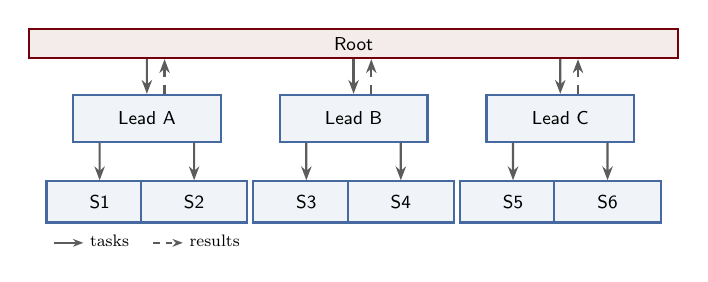
\begin{tikzpicture}[node distance=0.6cm and 0.6cm, scale=0.75, transform shape]
  \node[agentbox=garnet, minimum width=11cm, minimum height=0.5cm] (root) {Root};
  \node[agentbox=atlantic, minimum width=2.5cm] at ([yshift=-1cm, xshift=-3.5cm]root.south) (la) {Lead A};
  \node[agentbox=atlantic, minimum width=2.5cm] at ([yshift=-1cm]root.south) (lb) {Lead B};
  \node[agentbox=atlantic, minimum width=2.5cm] at ([yshift=-1cm, xshift=3.5cm]root.south) (lc) {Lead C};
  \draw[dataarrow] (root.south -| la) -- (la);
  \draw[dataarrow] (root.south -| lb) -- (lb);
  \draw[dataarrow] (root.south -| lc) -- (lc);
  \draw[dataarrow, dashed] ([xshift=0.3cm]la.north) -- ([xshift=0.3cm]root.south -| la);
  \draw[dataarrow, dashed] ([xshift=0.3cm]lb.north) -- ([xshift=0.3cm]root.south -| lb);
  \draw[dataarrow, dashed] ([xshift=0.3cm]lc.north) -- ([xshift=0.3cm]root.south -| lc);
  \node[workerbox] at ([yshift=-1cm, xshift=-0.8cm]la.south) (s1) {S1};
  \node[workerbox] at ([yshift=-1cm, xshift=0.8cm]la.south)  (s2) {S2};
  \node[workerbox] at ([yshift=-1cm, xshift=-0.8cm]lb.south) (s3) {S3};
  \node[workerbox] at ([yshift=-1cm, xshift=0.8cm]lb.south)  (s4) {S4};
  \node[workerbox] at ([yshift=-1cm, xshift=-0.8cm]lc.south) (s5) {S5};
  \node[workerbox] at ([yshift=-1cm, xshift=0.8cm]lc.south)  (s6) {S6};
  \draw[dataarrow] (la.south -| s1) -- (s1);
  \draw[dataarrow] (la.south -| s2) -- (s2);
  \draw[dataarrow] (lb.south -| s3) -- (s3);
  \draw[dataarrow] (lb.south -| s4) -- (s4);
  \draw[dataarrow] (lc.south -| s5) -- (s5);
  \draw[dataarrow] (lc.south -| s6) -- (s6);
  \node[font=\footnotesize, anchor=west] at ([yshift=-0.3cm]s1.south west) {%
    \tikz\draw[dataarrow] (0,0) -- (0.5,0); tasks \quad
    \tikz\draw[dataarrow, dashed] (0,0) -- (0.5,0); results};
\end{tikzpicture}

\vspace{0.2cm}
\small Tasks flow down, results flow up --- root never talks to specialists directly
\end{frame}

\begin{frame}{Unidirectional vs.\ Bidirectional Communication}
\centering
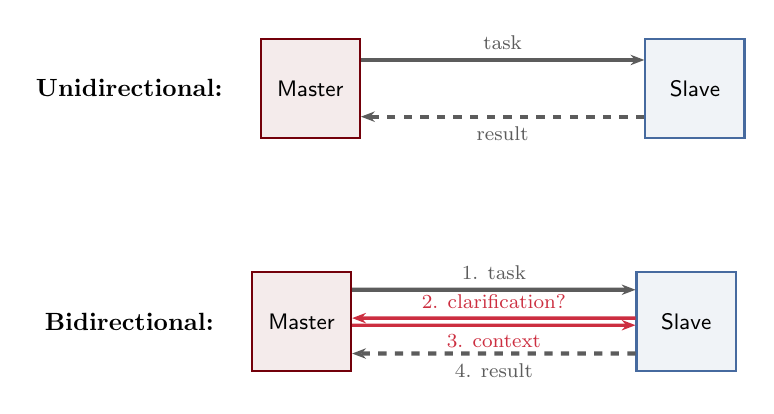
\begin{tikzpicture}[node distance=0.7cm and 1.2cm, scale=0.9, transform shape]
  % Unidirectional
  \node[font=\bfseries, anchor=east] (label1) {Unidirectional:};
  \node[agentbox=garnet, right=0.4cm of label1, minimum width=1.4cm, minimum height=1.4cm] (m1) {Master};
  \node[workerbox, right=4cm of m1, minimum width=1.4cm, minimum height=1.4cm] (w1) {Slave};
  \draw[dataarrow, line width=1.5pt] ([yshift=0.4cm]m1.east) -- node[above] {\footnotesize task} ([yshift=0.4cm]w1.west);
  \draw[dataarrow, dashed, line width=1.5pt] ([yshift=-0.4cm]w1.west) -- node[below] {\footnotesize result} ([yshift=-0.4cm]m1.east);

  % Bidirectional
  \node[font=\bfseries, anchor=east, below=2.8cm of label1] (label2) {Bidirectional:};
  \node[agentbox=garnet, right=0.4cm of label2, minimum width=1.4cm, minimum height=1.4cm] (m2) {Master};
  \node[workerbox, right=4cm of m2, minimum width=1.4cm, minimum height=1.4cm] (w2) {Slave};
  \draw[dataarrow, line width=1.5pt] ([yshift=0.45cm]m2.east) -- node[above] {\footnotesize 1. task} ([yshift=0.45cm]w2.west);
  \draw[dataarrow, dashed, line width=1.5pt] ([yshift=-0.45cm]w2.west) -- node[below] {\footnotesize 4. result} ([yshift=-0.45cm]m2.east);
  \draw[dataarrow=rose, line width=1.2pt] ([yshift=0.05cm]w2.west) -- node[above, pos=0.5] {\footnotesize\color{rose} 2. clarification?} ([yshift=0.05cm]m2.east);
  \draw[dataarrow=rose, line width=1.2pt] ([yshift=-0.05cm]m2.east) -- node[below, pos=0.5] {\footnotesize\color{rose} 3. context} ([yshift=-0.05cm]w2.west);
\end{tikzpicture}
\end{frame}

% ══════════════════════════════════════════════════════════
\section{Canonical Patterns}
% ══════════════════════════════════════════════════════════

\begin{frame}{Four Canonical Patterns}
\begin{itemize}
    \item \textbf{Pipeline:} Serial, single-pass, unidirectional
    \item \textbf{Fan-Out/Fan-In:} Parallel, single-pass, unidirectional
    \item \textbf{Master-Slave Pool:} Parallel, iterative, unidirectional
    \item \textbf{Feedback Loop:} Serial, iterative, bidirectional
\end{itemize}
\end{frame}

\begin{frame}{Pipeline Pattern}
\centering
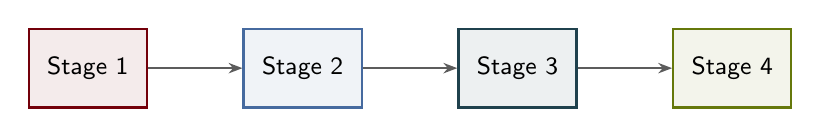
\begin{tikzpicture}[node distance=0.7cm and 1.0cm]
  \node[agentbox=garnet, minimum width=1.5cm, minimum height=1cm] (p1) {Stage 1};
  \node[agentbox=atlantic, right=1.2cm of p1, minimum width=1.5cm, minimum height=1cm] (p2) {Stage 2};
  \node[agentbox=congaree, right=1.2cm of p2, minimum width=1.5cm, minimum height=1cm] (p3) {Stage 3};
  \node[agentbox=horseshoe, right=1.2cm of p3, minimum width=1.5cm, minimum height=1cm] (p4) {Stage 4};
  \draw[dataarrow] (p1) -- (p2);
  \draw[dataarrow] (p2) -- (p3);
  \draw[dataarrow] (p3) -- (p4);
\end{tikzpicture}

\vspace{0.5cm}
\small Sequential transformation chain\\
Latency = sum of all stages
\end{frame}

\begin{frame}{Fan-Out/Fan-In Pattern}
\centering
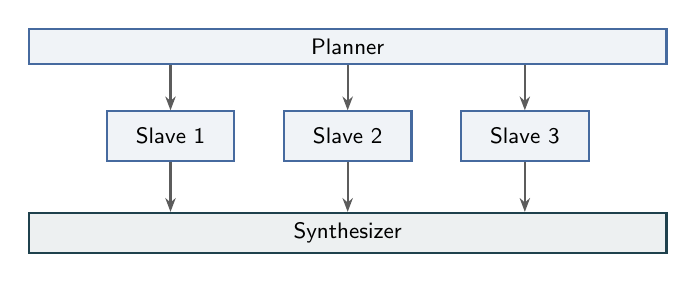
\begin{tikzpicture}[node distance=0.7cm and 1.0cm, scale=0.9, transform shape]
  \node[agentbox=atlantic, minimum width=9cm, minimum height=0.5cm] (planner) {Planner};
  \node[workerbox] at ([yshift=-1cm, xshift=-2.5cm]planner.south) (e1) {Slave 1};
  \node[workerbox] at ([yshift=-1cm]planner.south) (e2) {Slave 2};
  \node[workerbox] at ([yshift=-1cm, xshift=2.5cm]planner.south) (e3) {Slave 3};
  \draw[dataarrow] (planner.south -| e1) -- (e1);
  \draw[dataarrow] (planner.south -| e2) -- (e2);
  \draw[dataarrow] (planner.south -| e3) -- (e3);
  \node[agentbox=congaree, minimum width=9cm, minimum height=0.5cm] at ([yshift=-1cm]$(e1.south)!0.5!(e3.south)$) (syn) {Synthesizer};
  \draw[dataarrow] (e1) -- (syn.north -| e1);
  \draw[dataarrow] (e2) -- (syn.north -| e2);
  \draw[dataarrow] (e3) -- (syn.north -| e3);
\end{tikzpicture}

\vspace{0.3cm}
\small Independent subtasks in parallel\\
Latency = max of workers
\end{frame}

\begin{frame}{Master-Slave Pool Pattern}
\centering
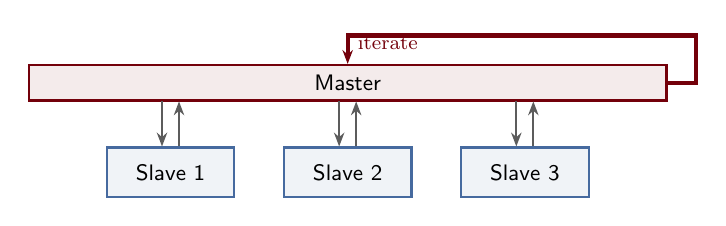
\begin{tikzpicture}[node distance=0.7cm and 1.0cm, scale=0.9, transform shape]
  \node[agentbox=garnet, minimum width=9cm, minimum height=0.5cm] (master) {Master};
  \node[workerbox] at ([yshift=-1cm, xshift=-2.5cm]master.south) (s1) {Slave 1};
  \node[workerbox] at ([yshift=-1cm]master.south) (s2) {Slave 2};
  \node[workerbox] at ([yshift=-1cm, xshift=2.5cm]master.south) (s3) {Slave 3};
  \draw[dataarrow] ([xshift=-0.12cm]master.south -| s1) -- ([xshift=-0.12cm]s1.north);
  \draw[dataarrow] ([xshift=0.12cm]s1.north) -- ([xshift=0.12cm]master.south -| s1);
  \draw[dataarrow] ([xshift=-0.12cm]master.south -| s2) -- ([xshift=-0.12cm]s2.north);
  \draw[dataarrow] ([xshift=0.12cm]s2.north) -- ([xshift=0.12cm]master.south -| s2);
  \draw[dataarrow] ([xshift=-0.12cm]master.south -| s3) -- ([xshift=-0.12cm]s3.north);
  \draw[dataarrow] ([xshift=0.12cm]s3.north) -- ([xshift=0.12cm]master.south -| s3);
  \draw[dataarrow, garnet, line width=1.5pt] (master.east) -- ++(0.4,0) |- ([yshift=0.4cm]master.north) -- (master.north) node[pos=0.25, right, font=\footnotesize] {iterate};
\end{tikzpicture}

\vspace{0.3cm}
\small Task queue + iterative processing\\
Best for batch workloads
\end{frame}

\begin{frame}{Feedback Loop Pattern}
\centering
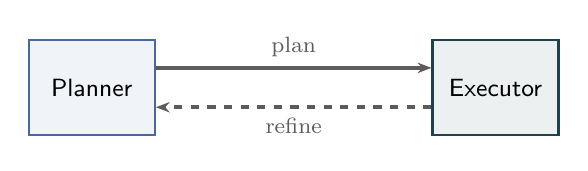
\begin{tikzpicture}[node distance=0.7cm and 1.0cm]
  \node[agentbox=atlantic, minimum width=1.6cm, minimum height=1.2cm] (planner) {Planner};
  \node[agentbox=congaree, right=3.5cm of planner, minimum width=1.6cm, minimum height=1.2cm] (executor) {Executor};
  \draw[dataarrow, line width=1.5pt] ([yshift=0.25cm]planner.east) -- node[above] {\footnotesize plan} ([yshift=0.25cm]executor.west);
  \draw[dataarrow, dashed, line width=1.5pt] ([yshift=-0.25cm]executor.west) -- node[below] {\footnotesize refine} ([yshift=-0.25cm]planner.east);
\end{tikzpicture}

\vspace{0.5cm}
\small Iterative refinement until quality threshold\\
Best for tasks requiring multiple attempts
\end{frame}

% ══════════════════════════════════════════════════════════
\section{Multi-Layered Architectures}
% ══════════════════════════════════════════════════════════

\begin{frame}{Why Multi-Layered?}
\begin{itemize}
    \item Flat master = bottleneck at scale
    \item Context fills with operational details
    \item Layering separates: Strategy $\to$ Planning $\to$ Execution
    \item Each layer filters and abstracts information
\end{itemize}
\end{frame}

\begin{frame}{Flat Architecture (Two-Layer)}
\centering
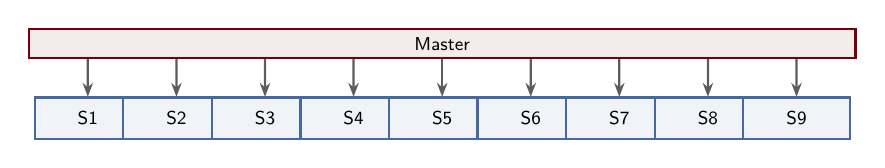
\begin{tikzpicture}[node distance=0.6cm and 0.6cm, scale=0.75, transform shape]
  \node[agentbox=garnet, minimum width=14cm, minimum height=0.5cm] (master) {Master};
  \node[workerbox] at ([yshift=-1cm, xshift=-6cm]master.south) (w1) {S1};
  \node[workerbox] at ([yshift=-1cm, xshift=-4.5cm]master.south) (w2) {S2};
  \node[workerbox] at ([yshift=-1cm, xshift=-3cm]master.south) (w3) {S3};
  \node[workerbox] at ([yshift=-1cm, xshift=-1.5cm]master.south) (w4) {S4};
  \node[workerbox] at ([yshift=-1cm]master.south) (w5) {S5};
  \node[workerbox] at ([yshift=-1cm, xshift=1.5cm]master.south) (w6) {S6};
  \node[workerbox] at ([yshift=-1cm, xshift=3cm]master.south) (w7) {S7};
  \node[workerbox] at ([yshift=-1cm, xshift=4.5cm]master.south) (w8) {S8};
  \node[workerbox] at ([yshift=-1cm, xshift=6cm]master.south) (w9) {S9};
  \foreach \w in {w1,w2,w3,w4,w5,w6,w7,w8,w9} { \draw[dataarrow] (master.south -| \w) -- (\w); }
\end{tikzpicture}

\vspace{0.3cm}
\small Master holds both strategic and tactical context\\
Context overload as slaves grow
\end{frame}

\begin{frame}{Layered Architecture (Three-Layer)}
\centering
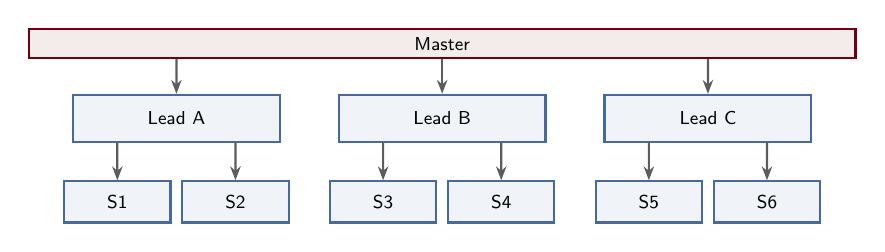
\begin{tikzpicture}[node distance=0.6cm and 0.6cm, scale=0.75, transform shape]
  \node[agentbox=garnet, minimum width=14cm, minimum height=0.5cm] (root) {Master};
  \node[agentbox=atlantic, minimum width=3.5cm] at ([yshift=-1cm, xshift=-4.5cm]root.south) (leadA) {Lead A};
  \node[agentbox=atlantic, minimum width=3.5cm] at ([yshift=-1cm]root.south) (leadB) {Lead B};
  \node[agentbox=atlantic, minimum width=3.5cm] at ([yshift=-1cm, xshift=4.5cm]root.south) (leadC) {Lead C};
  \draw[dataarrow] (root.south -| leadA) -- (leadA);
  \draw[dataarrow] (root.south -| leadB) -- (leadB);
  \draw[dataarrow] (root.south -| leadC) -- (leadC);
  \node[workerbox] at ([yshift=-1cm, xshift=-1cm]leadA.south) (sa1) {S1};
  \node[workerbox] at ([yshift=-1cm, xshift=1cm]leadA.south) (sa2) {S2};
  \node[workerbox] at ([yshift=-1cm, xshift=-1cm]leadB.south) (sb1) {S3};
  \node[workerbox] at ([yshift=-1cm, xshift=1cm]leadB.south) (sb2) {S4};
  \node[workerbox] at ([yshift=-1cm, xshift=-1cm]leadC.south) (sc1) {S5};
  \node[workerbox] at ([yshift=-1cm, xshift=1cm]leadC.south) (sc2) {S6};
  \draw[dataarrow] (leadA.south -| sa1) -- (sa1);
  \draw[dataarrow] (leadA.south -| sa2) -- (sa2);
  \draw[dataarrow] (leadB.south -| sb1) -- (sb1);
  \draw[dataarrow] (leadB.south -| sb2) -- (sb2);
  \draw[dataarrow] (leadC.south -| sc1) -- (sc1);
  \draw[dataarrow] (leadC.south -| sc2) -- (sc2);
\end{tikzpicture}

\vspace{0.3cm}
\small Each layer has smaller context budget\\
No single agent holds entire system state
\end{frame}

\begin{frame}{Deep vs.\ Wide Architecture}
\centering
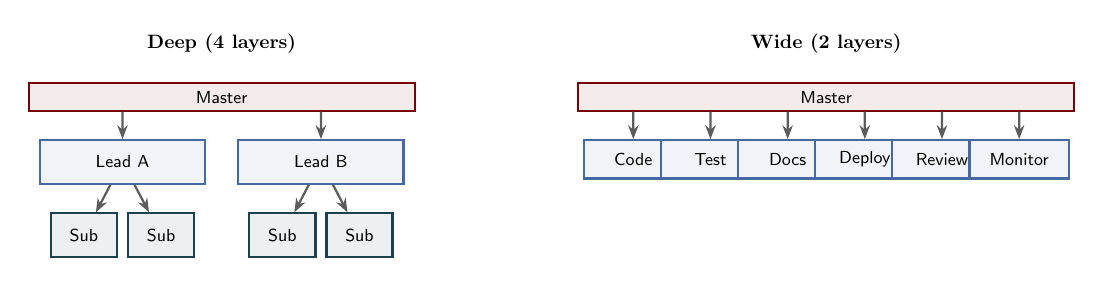
\begin{tikzpicture}[node distance=0.5cm and 0.5cm, scale=0.7, transform shape]
  % Deep
  \node[font=\bfseries] (deep-title) {Deep (4 layers)};
  \node[agentbox=garnet, minimum width=7cm, minimum height=0.4cm, below=0.4cm of deep-title] (dm) {Master};
  \node[agentbox=atlantic, minimum width=3cm, below=0.5cm of dm, xshift=-1.8cm] (dla) {Lead A};
  \node[agentbox=atlantic, minimum width=3cm, below=0.5cm of dm, xshift=1.8cm] (dlb) {Lead B};
  \draw[dataarrow] (dm.south -| dla) -- (dla);
  \draw[dataarrow] (dm.south -| dlb) -- (dlb);
  \node[agentbox=congaree, minimum width=1.2cm, below=0.5cm of dla, xshift=-0.7cm] (dsla1) {Sub};
  \node[agentbox=congaree, minimum width=1.2cm, below=0.5cm of dla, xshift=0.7cm] (dsla2) {Sub};
  \node[agentbox=congaree, minimum width=1.2cm, below=0.5cm of dlb, xshift=-0.7cm] (dslb1) {Sub};
  \node[agentbox=congaree, minimum width=1.2cm, below=0.5cm of dlb, xshift=0.7cm] (dslb2) {Sub};
  \draw[dataarrow] (dla) -- (dsla1);
  \draw[dataarrow] (dla) -- (dsla2);
  \draw[dataarrow] (dlb) -- (dslb1);
  \draw[dataarrow] (dlb) -- (dslb2);

  % Wide
  \node[font=\bfseries, right=8cm of deep-title] (wide-title) {Wide (2 layers)};
  \node[agentbox=garnet, minimum width=9cm, minimum height=0.4cm, below=0.4cm of wide-title] (wm) {Master};
  \node[workerbox, below=0.5cm of wm, xshift=-3.5cm] (ws1) {Code};
  \node[workerbox, below=0.5cm of wm, xshift=-2.1cm] (ws2) {Test};
  \node[workerbox, below=0.5cm of wm, xshift=-0.7cm] (ws3) {Docs};
  \node[workerbox, below=0.5cm of wm, xshift=0.7cm] (ws4) {Deploy};
  \node[workerbox, below=0.5cm of wm, xshift=2.1cm] (ws5) {Review};
  \node[workerbox, below=0.5cm of wm, xshift=3.5cm] (ws6) {Monitor};
  \foreach \s in {ws1,ws2,ws3,ws4,ws5,ws6} { \draw[dataarrow] (wm.south -| \s) -- (\s); }
\end{tikzpicture}

\vspace{0.3cm}
\small Deep: hierarchical refinement \quad Wide: domain coverage
\end{frame}

% ══════════════════════════════════════════════════════════
\section{Common Patterns in Practice}
% ══════════════════════════════════════════════════════════

\begin{frame}{Pipeline Pattern in Practice}
\centering
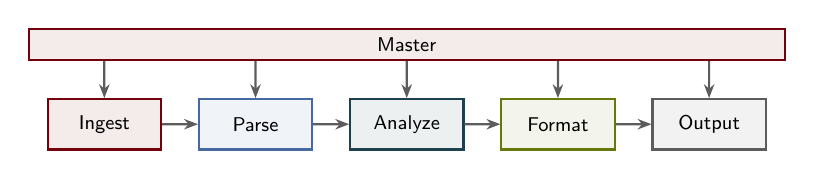
\begin{tikzpicture}[node distance=0.6cm and 0.6cm, scale=0.8, transform shape]
  \node[agentbox=garnet, minimum width=12cm, minimum height=0.5cm] (master) {Master};
  \node[agentbox=garnet, minimum width=1.8cm] at ([yshift=-1cm, xshift=-4.8cm]master.south) (ingest) {Ingest};
  \node[agentbox=atlantic, minimum width=1.8cm] at ([yshift=-1cm, xshift=-2.4cm]master.south) (parse) {Parse};
  \node[agentbox=congaree, minimum width=1.8cm] at ([yshift=-1cm]master.south) (analyze) {Analyze};
  \node[agentbox=horseshoe, minimum width=1.8cm] at ([yshift=-1cm, xshift=2.4cm]master.south) (format) {Format};
  \node[agentbox=bk70, minimum width=1.8cm] at ([yshift=-1cm, xshift=4.8cm]master.south) (output) {Output};
  \foreach \s in {ingest,parse,analyze,format,output} { \draw[dataarrow] (master.south -| \s) -- (\s); }
  \draw[dataarrow] (ingest) -- (parse);
  \draw[dataarrow] (parse) -- (analyze);
  \draw[dataarrow] (analyze) -- (format);
  \draw[dataarrow] (format) -- (output);
\end{tikzpicture}

\vspace{0.3cm}
\small Document processing: each stage transforms and forwards
\end{frame}

\begin{frame}{Fan-Out/Fan-In in Practice}
\centering
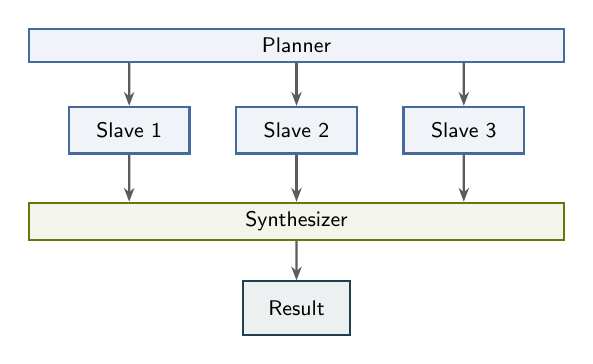
\begin{tikzpicture}[node distance=0.6cm and 0.6cm, scale=0.85, transform shape]
  \node[agentbox=atlantic, minimum width=8cm, minimum height=0.5cm] (planner) {Planner};
  \node[workerbox] at ([yshift=-1cm, xshift=-2.5cm]planner.south) (s1) {Slave 1};
  \node[workerbox] at ([yshift=-1cm]planner.south) (s2) {Slave 2};
  \node[workerbox] at ([yshift=-1cm, xshift=2.5cm]planner.south) (s3) {Slave 3};
  \draw[dataarrow] (planner.south -| s1) -- (s1);
  \draw[dataarrow] (planner.south -| s2) -- (s2);
  \draw[dataarrow] (planner.south -| s3) -- (s3);
  \node[agentbox=horseshoe, minimum width=8cm, minimum height=0.5cm] at ([yshift=-1cm]$(s1.south)!0.5!(s3.south)$) (synth) {Synthesizer};
  \draw[dataarrow] (s1) -- (synth.north -| s1);
  \draw[dataarrow] (s2) -- (synth.north -| s2);
  \draw[dataarrow] (s3) -- (synth.north -| s3);
  \node[agentbox=congaree, minimum width=1.6cm] at ([yshift=-1cm]synth.south) (result) {Result};
  \draw[dataarrow] (synth) -- (result);
\end{tikzpicture}

\vspace{0.3cm}
\small Literature review: parallel searches, merged bibliography
\end{frame}

\begin{frame}{Master-Slave Pool in Practice}
\centering
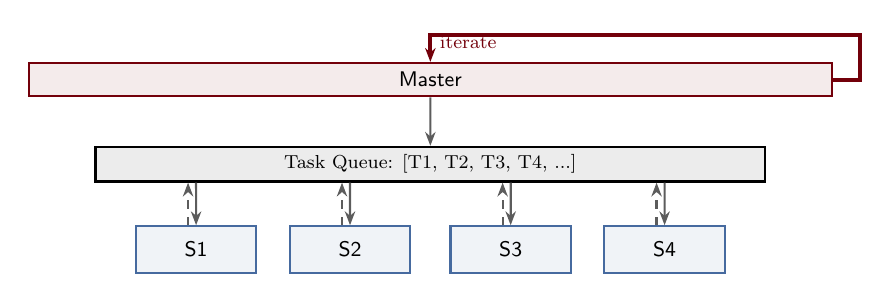
\begin{tikzpicture}[node distance=0.6cm and 0.6cm, scale=0.85, transform shape]
  \node[agentbox=garnet, minimum width=12cm, minimum height=0.5cm] (master) {Master};
  \node[draw=black, line width=1pt, fill=bk10, minimum width=10cm, minimum height=0.5cm, font=\footnotesize] at ([yshift=-1cm]master.south) (queue) {Task Queue: [T1, T2, T3, T4, ...]};
  \node[workerbox] at ([yshift=-1cm, xshift=-3.5cm]queue.south) (s1) {S1};
  \node[workerbox] at ([yshift=-1cm, xshift=-1.2cm]queue.south) (s2) {S2};
  \node[workerbox] at ([yshift=-1cm, xshift=1.2cm]queue.south) (s3) {S3};
  \node[workerbox] at ([yshift=-1cm, xshift=3.5cm]queue.south) (s4) {S4};
  \draw[dataarrow] (master) -- (queue);
  \draw[dataarrow] (queue.south -| s1) -- (s1);
  \draw[dataarrow] (queue.south -| s2) -- (s2);
  \draw[dataarrow] (queue.south -| s3) -- (s3);
  \draw[dataarrow] (queue.south -| s4) -- (s4);
  \draw[dataarrow, dashed] ([xshift=-0.12cm]s1.north) -- ([xshift=-0.12cm]queue.south -| s1);
  \draw[dataarrow, dashed] ([xshift=-0.12cm]s2.north) -- ([xshift=-0.12cm]queue.south -| s2);
  \draw[dataarrow, dashed] ([xshift=-0.12cm]s3.north) -- ([xshift=-0.12cm]queue.south -| s3);
  \draw[dataarrow, dashed] ([xshift=-0.12cm]s4.north) -- ([xshift=-0.12cm]queue.south -| s4);
  \draw[dataarrow, garnet, line width=1.5pt] (master.east) -- ++(0.4,0) |- ([yshift=0.4cm]master.north) -- (master.north) node[pos=0.25, right, font=\footnotesize] {iterate};
\end{tikzpicture}

\vspace{0.2cm}
\small Batch processing: slaves pull tasks, results may generate new tasks
\end{frame}

\begin{frame}{Feedback Loop in Practice}
\centering
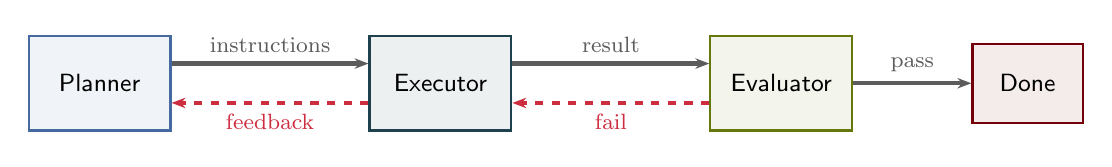
\begin{tikzpicture}[node distance=0.7cm and 1.0cm]
  \node[agentbox=atlantic, minimum width=1.8cm, minimum height=1.2cm] (planner) {Planner};
  \node[agentbox=congaree, right=2.5cm of planner, minimum width=1.8cm, minimum height=1.2cm] (executor) {Executor};
  \node[agentbox=horseshoe, right=2.5cm of executor, minimum width=1.8cm, minimum height=1.2cm] (evaluator) {Evaluator};
  \node[agentbox=garnet, right=1.5cm of evaluator, minimum width=1.4cm, minimum height=1cm] (done) {Done};
  \draw[dataarrow, line width=1.5pt] ([yshift=0.25cm]planner.east) -- node[above] {\footnotesize instructions} ([yshift=0.25cm]executor.west);
  \draw[dataarrow, line width=1.5pt] ([yshift=0.25cm]executor.east) -- node[above] {\footnotesize result} ([yshift=0.25cm]evaluator.west);
  \draw[dataarrow, line width=1.5pt] (evaluator.east) -- node[above] {\footnotesize pass} (done.west);
  \draw[dataarrow=rose, dashed, line width=1.5pt] ([yshift=-0.25cm]evaluator.west) -- node[below] {\footnotesize\color{rose} fail} ([yshift=-0.25cm]executor.east);
  \draw[dataarrow=rose, dashed, line width=1.5pt] ([yshift=-0.25cm]executor.west) -- node[below] {\footnotesize\color{rose} feedback} ([yshift=-0.25cm]planner.east);
\end{tikzpicture}

\vspace{0.3cm}
\small Code generation: write $\to$ test $\to$ fix $\to$ repeat
\end{frame}

\begin{frame}{Composite Workflow Example}
\centering
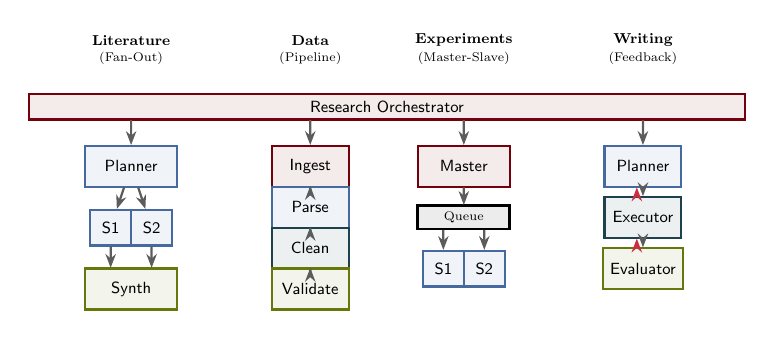
\begin{tikzpicture}[node distance=0.5cm and 0.5cm, scale=0.65, transform shape]
  % Labels
  \node[font=\footnotesize\bfseries] at (-5,1.3) {Literature};
  \node[font=\scriptsize] at (-5,0.95) {(Fan-Out)};
  \node[font=\footnotesize\bfseries] at (-1.5,1.3) {Data};
  \node[font=\scriptsize] at (-1.5,0.95) {(Pipeline)};
  \node[font=\footnotesize\bfseries] at (1.5,1.3) {Experiments};
  \node[font=\scriptsize] at (1.5,0.95) {(Master-Slave)};
  \node[font=\footnotesize\bfseries] at (5,1.3) {Writing};
  \node[font=\scriptsize] at (5,0.95) {(Feedback)};

  % Orchestrator
  \node[agentbox=garnet, minimum width=14cm, minimum height=0.5cm] (orch) {Research Orchestrator};

  % Literature
  \node[agentbox=atlantic, minimum width=1.8cm] at ([yshift=-0.9cm, xshift=-5cm]orch.south) (lit_plan) {Planner};
  \node[workerbox, minimum width=0.8cm] at ([yshift=-2.1cm, xshift=-5.4cm]orch.south) (l1) {S1};
  \node[workerbox, minimum width=0.8cm] at ([yshift=-2.1cm, xshift=-4.6cm]orch.south) (l2) {S2};
  \node[agentbox=horseshoe, minimum width=1.8cm] at ([yshift=-3.3cm, xshift=-5cm]orch.south) (lit_merge) {Synth};
  \draw[dataarrow] (orch.south -| lit_plan) -- (lit_plan);
  \draw[dataarrow] (lit_plan) -- (l1);
  \draw[dataarrow] (lit_plan) -- (l2);
  \draw[dataarrow] (l1) -- (lit_merge.north -| l1);
  \draw[dataarrow] (l2) -- (lit_merge.north -| l2);

  % Data
  \node[agentbox=garnet, minimum width=1.5cm] at ([yshift=-0.9cm, xshift=-1.5cm]orch.south) (d1) {Ingest};
  \node[agentbox=atlantic, minimum width=1.5cm] at ([yshift=-1.7cm, xshift=-1.5cm]orch.south) (d2) {Parse};
  \node[agentbox=congaree, minimum width=1.5cm] at ([yshift=-2.5cm, xshift=-1.5cm]orch.south) (d3) {Clean};
  \node[agentbox=horseshoe, minimum width=1.5cm] at ([yshift=-3.3cm, xshift=-1.5cm]orch.south) (d4) {Validate};
  \draw[dataarrow] (orch.south -| d1) -- (d1);
  \draw[dataarrow] (d1) -- (d2);
  \draw[dataarrow] (d2) -- (d3);
  \draw[dataarrow] (d3) -- (d4);

  % Experiments
  \node[agentbox=garnet, minimum width=1.8cm] at ([yshift=-0.9cm, xshift=1.5cm]orch.south) (exp_master) {Master};
  \node[draw=black, line width=1pt, fill=bk10, minimum width=1.8cm, minimum height=0.4cm, font=\scriptsize] at ([yshift=-1.9cm, xshift=1.5cm]orch.south) (exp_queue) {Queue};
  \node[workerbox, minimum width=0.8cm] at ([yshift=-2.9cm, xshift=1.1cm]orch.south) (e1) {S1};
  \node[workerbox, minimum width=0.8cm] at ([yshift=-2.9cm, xshift=1.9cm]orch.south) (e2) {S2};
  \draw[dataarrow] (orch.south -| exp_master) -- (exp_master);
  \draw[dataarrow] (exp_master) -- (exp_queue);
  \draw[dataarrow] (exp_queue.south -| e1) -- (e1);
  \draw[dataarrow] (exp_queue.south -| e2) -- (e2);

  % Writing
  \node[agentbox=atlantic, minimum width=1.5cm] at ([yshift=-0.9cm, xshift=5cm]orch.south) (w_plan) {Planner};
  \node[agentbox=congaree, minimum width=1.5cm] at ([yshift=-1.9cm, xshift=5cm]orch.south) (w_exec) {Executor};
  \node[agentbox=horseshoe, minimum width=1.5cm] at ([yshift=-2.9cm, xshift=5cm]orch.south) (w_eval) {Evaluator};
  \draw[dataarrow] (orch.south -| w_plan) -- (w_plan);
  \draw[dataarrow] (w_plan) -- (w_exec);
  \draw[dataarrow] (w_exec) -- (w_eval);
  \draw[dataarrow=rose, dashed] ([xshift=-0.12cm]w_eval.north) -- ([xshift=-0.12cm]w_exec.south);
  \draw[dataarrow=rose, dashed] ([xshift=-0.12cm]w_exec.north) -- ([xshift=-0.12cm]w_plan.south);
\end{tikzpicture}

\vspace{0.2cm}
\small Real systems combine multiple patterns
\end{frame}

% ══════════════════════════════════════════════════════════
\section{Pattern Selection}
% ══════════════════════════════════════════════════════════

\begin{frame}{Pattern Selection Guide}
\centering
\small
\begin{tabular}{lcccc}
\toprule
\textbf{Criterion} & \textbf{Pipeline} & \textbf{Fan-Out} & \textbf{Master-Slave} & \textbf{Feedback} \\
\midrule
Independence & Low & High & High & Low \\
Iteration & No & No & Optional & Yes \\
Scale & 3--5 & 3--20 & 10--100+ & 2--5 \\
Latency & Sum & Max & Batched & Iterations \\
Best for & Transforms & Parallel work & Batch & Refinement \\
\bottomrule
\end{tabular}
\end{frame}

\begin{frame}{Agent Architecture Taxonomy}
\centering
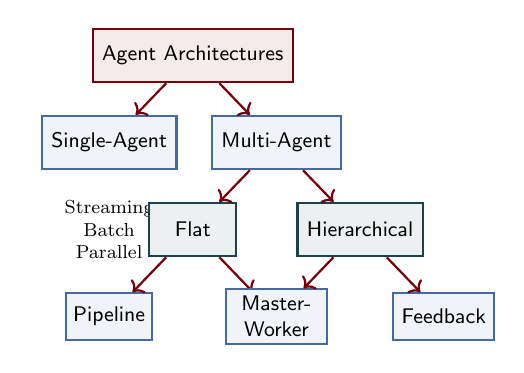
\begin{tikzpicture}[
  level distance=1.3cm,
  sibling distance=2.5cm,
  edge from parent/.style={draw, garnet, thick, ->},
  every node/.style={font=\small},
  scale=0.85, transform shape
]
\node[agentbox=garnet, minimum width=2.2cm] {Agent Architectures}
  child {
    node[agentbox=atlantic, minimum width=1.8cm] {Single-Agent}
    child {
      node[font=\footnotesize, text width=2.2cm, align=center] {Streaming\\Batch\\Parallel}
      edge from parent[draw=none]
    }
  }
  child {
    node[agentbox=atlantic, minimum width=1.8cm] {Multi-Agent}
    child {
      node[agentbox=congaree, minimum width=1.3cm] {Flat}
      child { node[workerbox, minimum width=1.1cm] {Pipeline} }
      child { node[workerbox, minimum width=1.1cm, text width=1.3cm, align=center] {Fan-Out} }
    }
    child {
      node[agentbox=congaree, minimum width=1.3cm] {Hierarchical}
      child { node[workerbox, minimum width=1.1cm, text width=1.3cm, align=center] {Master-\\Worker} }
      child { node[workerbox, minimum width=1.1cm, text width=1.3cm, align=center] {Feedback} }
    }
  };
\end{tikzpicture}
\end{frame}

% ══════════════════════════════════════════════════════════
\section{Conclusion}
% ══════════════════════════════════════════════════════════

\begin{frame}{Key Takeaways}
\begin{itemize}
    \item LLM is an uncommitted tool --- power comes from composition
    \item Four canonical patterns: Pipeline, Fan-Out, Master-Slave, Feedback Loop
    \item Architecture emerges from task structure, not model capability
    \item Patterns are composable --- real systems combine them
    \item Multi-layered hierarchies scale beyond single-agent limits
\end{itemize}
\end{frame}

\begin{frame}{}
\centering
\vspace{2cm}
{\Huge\textcolor{garnet}{Questions?}}
\vspace{1cm}

\small
J.C.\ Vaught\\
\texttt{jvaught@sc.edu}\\
University of South Carolina
\end{frame}

\end{document}
